% !TEX root = ../main.tex

\section{Limits}

\begin{myframe}[arc=10pt,auto outer arc]

\begin{enumerate}
\item One sided limits:
	\begin{enumerate}
		\item the limit of $f(x)$ as $x$ approaches $a$ from the right is $L$.
		\[
			\lim_{x\rightarrow a^+} f\left(x\right) = L
		\]
		\item the limit of $f(x)$ as $x$ approaches $a$ from the left is $L$.
		\[
			\lim_{x\rightarrow a^-} f\left(x\right) = L
		\]		
	\end{enumerate}
\item Two sided limits:

    \begin{enumerate}
    \item What is the limit of the following function as x approaches a?
    \[
    	\lim_{x\rightarrow a} f\left(x\right) = L \iff \lim_{x\rightarrow a^-} f\left(x\right) = \lim_{x\rightarrow a^+} f\left(x\right) = L
    \]
    
    \item If there is no sign in the limit notation, then you’re being asked for a two-sided limit. You only have a two-sided limit if your left and right limits agree. The existence of a limit from the left-hand side does not imply that you have a right-sided limit.
    When we say that something has a limit, then we mean that it has an actual numeric value.
    \end{enumerate}
    
\item Infinite limits
	\begin{enumerate}
		\item Increases without bound
		\[ \lim_{x \rightarrow a} f(x) = +\infty \]
		\item Decreases without bound
		\[ \lim_{x \rightarrow a} f(x) = -\infty \]
	\end{enumerate}

\item Limits at infinity
	\begin{enumerate}
	\item $\displaystyle \lim_{x \rightarrow +\infty} f(x) = L$: $\displaystyle f(x) \rightarrow L \textrm{ as } x \rightarrow +\infty$
	\item $\displaystyle \lim_{x \rightarrow -\infty} f(x) = L$: $\displaystyle f(x) \rightarrow L \textrm{ as } x \rightarrow -\infty$
	\end{enumerate}

\item Vertical asymptote

If $\displaystyle \left( \lim_{x\rightarrow a^-} f\left(x\right) = +\infty \textrm{ or } 
 \lim_{x\rightarrow a^-} f\left(x\right) = -\infty \right)$
and 
$\displaystyle \left( \lim_{x\rightarrow a^+} f\left(x\right) = +\infty  \textrm{ or }  
 \lim_{x\rightarrow a^+} f\left(x\right) = -\infty \right)$,
 
 then \textbf{the line $x=a$} is called the \textbf{vertical asymptote} of
 the graph of a function $f$.
 
 \item Horizontal asymptote
If  $\displaystyle \lim_{x\rightarrow +\infty} f\left(x\right) = L$ or $\displaystyle \lim_{x\rightarrow -\infty} f\left(x\right) = L$, then \textbf{the line $y=L$} is called the \textbf{horizontal asymptote} of the graph of a function f

\end{enumerate}

\end{myframe}

\newpage
\noindent Consider the graph of a function %f(x)$ below:

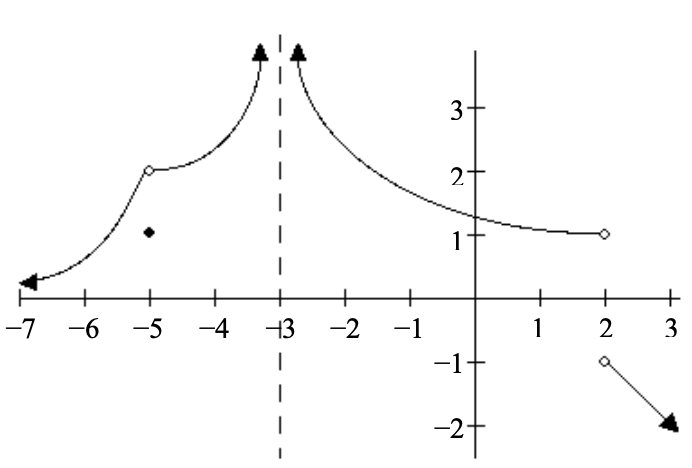
\includegraphics[width=0.7\linewidth]{chapter1/limits}

\noindent Find:

\pairofprobsans%
{$\displaystyle f(2)$}{undefined}
{$\displaystyle \lim_{x \rightarrow 2^-} f(x)$}{$\displaystyle 1$}

\pairofprobsans%
{$\displaystyle \lim_{x \rightarrow 2^+} f(x)$}{$\displaystyle -1$}
{$\displaystyle \lim_{x \rightarrow 2} f(x)$}{undefined}

\pairofprobsans%
{$\displaystyle f(-5)$}{$\displaystyle 1$}
{$\displaystyle \lim_{x \rightarrow -5^-} f(x)$}{$\displaystyle 2$}

\pairofprobsans%
{$\displaystyle \lim_{x \rightarrow -5^+} f(x)$}{$\displaystyle 2$}
{$\displaystyle \lim_{x \rightarrow -5} f(x)$}{$\displaystyle 2$}

\pairofprobsans%
{$\displaystyle f(-3)$}{undefined}
{$\displaystyle \lim_{x \rightarrow -3^-} f(x) $}{$\displaystyle +\infty$}

\pairofprobsans%
{$\displaystyle \lim_{x \rightarrow -3^+} f(x)$}{$\displaystyle +\infty$}
{$\displaystyle \lim_{x \rightarrow -3} f(x)$}{$\displaystyle +\infty$}

\pairofprobsans%
{$\displaystyle \lim_{x \rightarrow -\infty} f(x)$}{$\displaystyle 0$}
{$\displaystyle \lim_{x \rightarrow +\infty} f(x)$}{$\displaystyle -\infty$}

\problemans%
{The vertical asymptote}{$\displaystyle x=-3$}


